\begin{figure}[H]
    \centering
    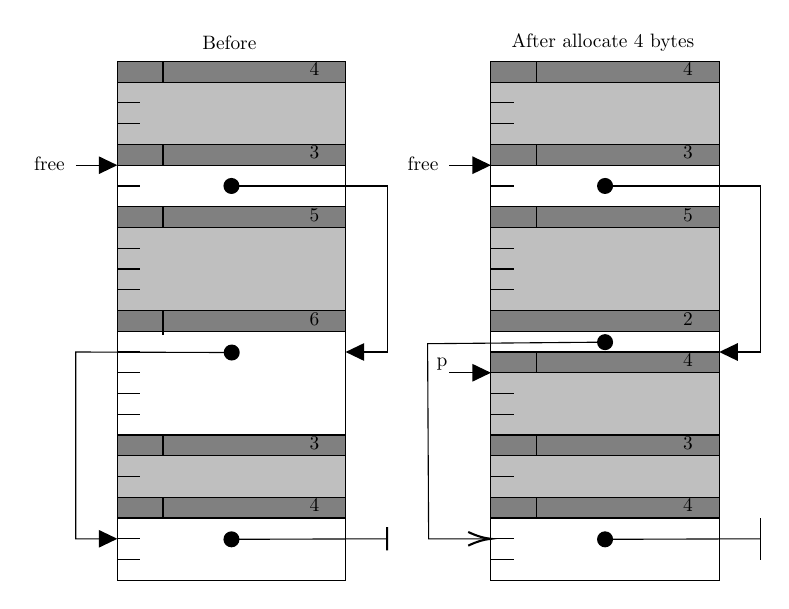
\begin{tikzpicture}[x=0.75pt,y=0.75pt,yscale=-1,xscale=1]
        \foreach \x in {20,60,90,140,200,230}{
            \draw  [fill=gray  ,fill opacity=1 ] (100,\x) -- (210,\x) -- (210,\x+10) -- (100,\x+10) -- cycle ;
        }
        
        \draw  [fill=lightgray  ,fill opacity=1 ] (100,30) -- (210,30) -- (210,60) -- (100,60) -- cycle ;
        \draw  [fill=white ,fill opacity=1 ] (100,70) -- (210,70) -- (210,90) -- (100,90) -- cycle ;
        \draw  [fill=lightgray ,fill opacity=1 ] (100,100) -- (210,100) -- (210,140) -- (100,140) -- cycle ;
        \draw  [fill=white  ,fill opacity=1 ] (100,150) -- (210,150) -- (210,200) -- (100,200) -- cycle ;
        \draw  [fill=lightgray  ,fill opacity=1 ] (100,210) -- (210,210) -- (210,230) -- (100,230) -- cycle ;
        \draw  [fill=white  ,fill opacity=1 ] (100,240) -- (210,240) -- (210,270) -- (100,270) -- cycle ;
        
        \foreach \x in {20,60,90,140,160,200,230}{
            \draw  [fill=gray  ,fill opacity=1 ] (280,\x) -- (390,\x) -- (390,\x+10) -- (280,\x+10) -- cycle ;
        }

        \draw  [fill=lightgray  ,fill opacity=1 ] (280,30) -- (390,30) -- (390,60) -- (280,60) -- cycle ;
        \draw  [fill=white  ,fill opacity=1 ] (280,70) -- (390,70) -- (390,90) -- (280,90) -- cycle ;
        \draw  [fill=lightgray  ,fill opacity=1 ] (280,100) -- (390,100) -- (390,140) -- (280,140) -- cycle ;
        \draw  [fill=white  ,fill opacity=1 ] (280,150) -- (390,150) -- (390,160) -- (280,160) -- cycle ;
        \draw  [fill=lightgray  ,fill opacity=1 ] (280,210) -- (390,210) -- (390,230) -- (280,230) -- cycle ;
        \draw  [fill=white  ,fill opacity=1 ] (280,240) -- (390,240) -- (390,270) -- (280,270) -- cycle ;
        \draw  [fill=lightgray ,fill opacity=1 ] (280,170) -- (390,170) -- (390,200) -- (280,200) -- cycle ;

        \foreach \x in {40,50,...,260}{
            \draw    (100,\x) -- (111,\x) ;
            \draw    (280,\x) -- (291,\x) ;
        }        
        
        \foreach \x in {20,60,90,160,200,230}{ \draw    (302,\x) -- (302,\x+10) ; }
        \foreach \x in {20,60,90,200,230}{ \draw    (122,\x) -- (122,\x+10) ; }
        
        \draw  (260,170) -- (278,170) ;
        \draw  (80,70) -- (98,70) ;
        \draw  (155,250.25) -- (230,250) ;
        \draw  (335,250.25) -- (410,250) ;
        \draw  (410,240) -- (410,260) ;        
        \draw  (260,70) -- (278,70) ;
        \draw  (122,140) -- (122,152) ;
        \draw  (155,80) -- (230,80) -- (230,160) -- (212,160) ;
        \draw  (335,155.25) -- (249.5,156) -- (250,250) -- (278,250) ;
        \draw  (335,80) -- (410,80) -- (410,160) -- (392,160) ;
        \draw  (155.13,160.25) -- (80,160) -- (80,250) -- (98,250) ;
        
        \draw [shift={(210,160)}, rotate = 360] [fill=black  ][line width=0.75]  [draw opacity=0] (8.93,-4.29) -- (0,0) -- (8.93,4.29) -- cycle;
        \draw [shift={(155,80)}, rotate = 0] [color=black  ][fill=black  ][line width=0.75] (0, 0) circle [x radius= 3.35, y radius= 3.35];
        \draw [shift={(100,250)}, rotate = 180] [fill=black  ][line width=0.75]  [draw opacity=0] (8.93,-4.29) -- (0,0) -- (8.93,4.29) -- cycle;
        \draw [shift={(155.13,160.25)}, rotate = 180.19] [color=black][fill=black ][line width=0.75](0, 0) circle [x radius= 3.35, y radius= 3.35];
        \draw [shift={(100,70)}, rotate = 180] [fill=black  ][line width=0.75]  [draw opacity=0] (8.93,-4.29) -- (0,0) -- (8.93,4.29) -- cycle;
        \draw [shift={(230,250)}, rotate = 539.81] [color=black  ][line width=0.75]    (0,5.59) -- (0,-5.59);
        \draw [shift={(155,250.25)}, rotate = 359.81] [color=black][fill=black ][line width=0.75] (0, 0) circle [x radius= 3.35, y radius= 3.35];
        \draw [shift={(390,160)}, rotate = 360] [fill=black ][line width=0.75]  [draw opacity=0] (8.93,-4.29) -- (0,0) -- (8.93,4.29) -- cycle;
        \draw [shift={(335,80)}, rotate = 0] [color=black ][fill=black ][line width=0.75] (0, 0) circle [x radius= 3.35, y radius= 3.35];
        \draw [shift={(280,70)}, rotate = 180] [fill=black ][line width=0.75]  [draw opacity=0] (8.93,-4.29) -- (0,0) -- (8.93,4.29) -- cycle;
        \draw [shift={(335,250.25)}, rotate = 359.81] [color=black][fill=black ][line width=0.75] (0, 0) circle [x radius= 3.35, y radius= 3.35];
        \draw [shift={(280,170)}, rotate = 180] [fill=black ][line width=0.75] [draw opacity=0] (8.93,-4.29) -- (0,0) -- (8.93,4.29) -- cycle;
        \draw [shift={(280,250)}, rotate = 180] [color=black ][line width=0.75] (10.93,-3.29) .. controls (6.95,-1.4) and (3.31,-0.3) .. (0,0) .. controls (3.31,0.3) and (6.95,1.4) .. (10.93,3.29);
        \draw [shift={(335,155.25)}, rotate = 179.5] [color=black ][fill=black ][line width=0.75] (0, 0) circle [x radius= 3.35, y radius= 3.35];
        
        \draw (67.33,69.33) node [scale=0.7] [align=left] {free};
        \draw (247.33,69.33) node [scale=0.7] [align=left] {free};
        \draw (256.5,166) node [scale=0.7] [align=left] {p};
        \draw (154,11) node [scale=0.7] [align=left] {Before};
        \draw (334,11) node [scale=0.7] [align=left] {After allocate 4 bytes};
        
        \foreach \x/\y in {24/4,64/3,94/5,144/6,204/3,234/4}{ \draw (195,\x) node [scale=0.7] [align=left] {\y}; }
        \foreach \x/\y in {24/4,64/3,94/5,144/2,164/4,204/3,234/4}{ \draw (375,\x) node [scale=0.7] [align=left] {\y}; }
    \end{tikzpicture}
    \caption{First-fit allocation policy}
    \label{fig:memman}
\end{figure}